%%%%%%%%%%%%%%%%%%%%%%%%%%%%%%%%%%%%%%%%%%%%%%%%%%%%%%%%%%%%%%%%%%%%%%%%%%%%%%%%%%%%%%%%%%%%%%%%%%%%%%%%%%%%%%%%%%%%%%%%%%%%%%
%2345678901234567890123456789012345678901234567890123456789012345678901234567890
%        1         2         3         4         5         6         7         8

\documentclass[letterpaper, 10 pt, conference]{ieeeconf}  
% Comment this line out if you need a4paper

%\documentclass[a4paper, 10pt, conference]{ieeeconf}      
% Use this line for a4 paper

\IEEEoverridecommandlockouts       % This command is only
                                                          % needed if you want to
                                                          % use the \thanks command
\overrideIEEEmargins
% See the \addtolength command later in the file to balance the column lengths
% on the last page of the document

% The following packages can be found on http:\\www.ctan.org
\usepackage{graphics} % for pdf, bitmapped graphics files
\usepackage{epsfig} % for postscript graphics files
\usepackage{mathptmx} % assumes new font selection scheme installed
\usepackage{times} % assumes new font selection scheme installed
%\usepackage{amsmath} % assumes amsmath package installed
%\usepackage{amssymb}  % assumes amsmath package installed
\usepackage{hyperref}
\usepackage{lipsum}
\usepackage{pythonhighlight}
\usepackage{textcomp}

\title{\LARGE \bf
Generating Musical Notes and Transcription using Deep Learning$^{*}$}

\author{Varad Meru$^{\#}$% <-this % stops a space
\\ {\small Student \# 26648958}
\thanks{$^{*}$This work was done as a part of the project for the course CS 274c: Neural Networks and Deep Learning, taught in Winter 2015 by Prof. Pierre Baldi at University of California, Irvine.}% <-this % stops a space
\thanks{$^{\#}$Dept. of Computer Science, Donald Bren School of Information and Computer Science, University of California, Irvine, email: {\tt\small vmeru@ics.uci.edu}}%
}

\begin{document}
\maketitle
\thispagestyle{empty}
\pagestyle{empty}

%%%%%%%%%%%%%%%%%%%%%%%%%%%%%%%%%%%%%%%%%%%%%%%%%%%%%%%%%%%%%%%%%%%%%%%%%%%%%%%%%%%%%%%%%%%%%%%%%%%%%%%%%%%%%%%%%%%%%%%%%%%%%%
\begin{abstract}
In recent years, deep learning approaches for building unsupervised hierarchical representations from unlabeled data have gained significant interest. Progress in fields, such as image processing and natural language processing, has been substantial, but to my knowledge, methods on auditory data for learning representations have not been studied extensively. 
\end{abstract}
%%%%%%%%%%%%%%%%%%%%%%%%%%%%%%%%%%%%%%%%%%%%%%%%%%%%%%%%%%%%%%%
%%%%%%%%%%%%%%%%%%%%%%%%%%%%%%%%%%%%%%%%%%%%%%%%%%%%%%%%%%%%%%%
\section{Introduction}

Tasks such such as object identification in an image or completing a sentence based on the context, which humans start doing from a very early age, are very challenging for a machine to perform as the formulation of these tasks into a set of steps is very complicated. The approaches till now were focussed more on the statistical properties of the corpus and thus, the features of the data were required to be hand engineered. This gave us good results, but hand-engineering of features was extremely complicated process for very large, unstructured and complex data such as images, speech, text corpus. Recent advances in deep learning have shown huge progress in solving these problems by focusing on generating the abstract features from the data, especially in the fields of image processing and natural language processing, but not much has been done in the field of audio signals. 

This project is an attempt to understand auditory signals better using deep learning methods and using that knowledge to generate music by learning from various sources of audio signals. There are two parts of this project: Understanding the temporal dependencies in a polyphonic music using the generalization of the RTRBM, called RNN-RBM\cite{c8}, to generate music from polyphonic MIDI tones, and, Apply the theory of Convolutional Deep-Belief networks\cite{c1} to learn abstract representations of the low-level description of audio signals such as STFTs and Chroma and recreating it. This work is inspired from AARON, the painter,\cite{c5} and the idea of machine doing art, which is one of the most abstract representations of human understanding, and from the work done by Tristan Jehan\cite{c4} on music synthesis using lower-level features of audio signals

Many music information retrieval (MIR) tasks depend on the extraction of low-level acoustic features. These features are usually constructed using task-dependent signal processing techniques. There are many features which are potentially useful for working with music: spectral, timbral, temporal, harmonic, etc (see \cite{c3} for a good review of features). This project tries to analyze these features and apply in the context of music synthesis. 

The remainder of the paper is organized as follows. In Sections 2, the preliminaries of the work are described. In 3 and 4, the RNN-RBM based architecture and the convolutional deep belief network (CDBN) approach to music understanding and synthesis is described. In Section 5, the datasets are described. In Section 6, I present the results on musical sequences and transcription.

%%%%%%%%%%%%%%%%%%%%%%%%%%%%%%%%%%%%%%%%%%%%%%%%%%%%%%%%%%%%%%%
%%%%%%%%%%%%%%%%%%%%%%%%%%%%%%%%%%%%%%%%%%%%%%%%%%%%%%%%%%%%%%%
\section{Preliminaries}
This section describes the preliminaries used in the project. 
\subsection{Restricted Boltzmann machines}
An RBM is an energy-based model where the joint probability of a given configuration of the visible vector $v$ (inputs) and the hidden vector $h$ is:
\begin{equation}
P(v,h) = \exp(-b_v^\textrm{T} v -b_v^\textrm{T} -h^\textrm{T}Wv )/Z
\end{equation}

where $b_v$, $b_h$ and $W$ are the model parameters and $Z$ is the usually intractable partition function. When the vector $v$ is given, the hidden units $h_i$ are conditionally independent of one another, and vice versa: 
\begin{equation}
P(h_i = 1 | v) = \sigma(b_h + W_v)_i
\end{equation}
\begin{equation}
P(v_j = 1 | h) = \sigma(b_v + W^\textrm{T} h)_j
\end{equation}
Where $\sigma(x) \equiv(1 + e^{-x})^{-1}$ is the logistic sigmoid function.

Inference in RBMs consists of sampling the $h_i$ given $v$, or vice versa, according to their Bernoulli distribution (given in eq. 2). Sampling $v$ can be performed efficiently by block Gibbs sampling. The gradient of the negative log likelihood of an input vector can be estimated by a single visible sample obtained from a $k$-step Gibbs chain starting $v^{(l)}$, resulting in the contrastive divergence algorithm\cite{c9}.%

\subsection{Music Information Retrieval}

\begin{figure}[thpb]
      \centering
      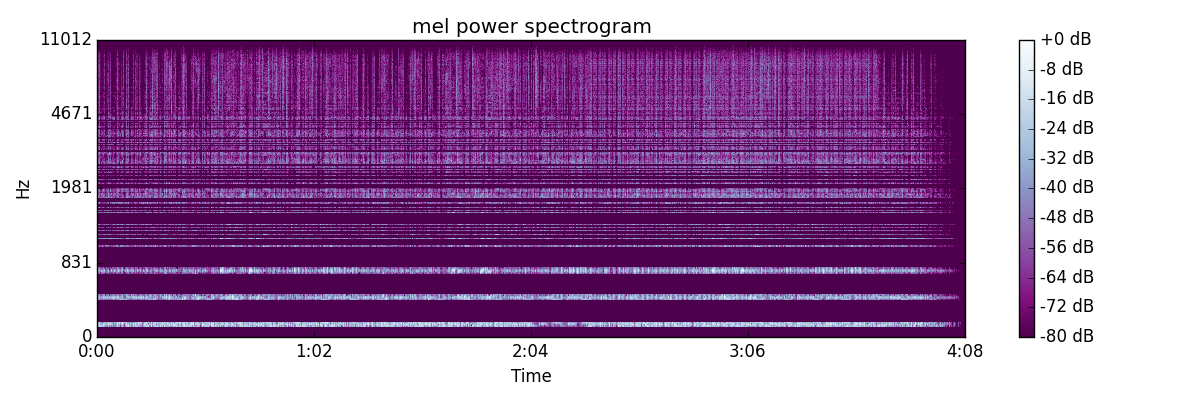
\includegraphics[scale=0.25]{mel_getlucky_3000_mels.png}
      \caption{Inductance of oscillation winding on amorphous
       magnetic core versus DC bias magnetic field}
      \label{figurelabel}
\end{figure}
%%%%%%%%%%%%%%%%%%%%%%%%%%%%%%%%%%%%%%%%%%%%%%%%%%%%%%%%%%%%
%%%%%%%%%%%%%%%%%%%%%%%%%%%%%%%%%%%%%%%%%%%%%%%%%%%%%%%%%%%%
\section{Methodology}
AAA

\section{Programming Details} 
AAA

\section{Datasets}
The datasets that were used for the experiments were: (1) A collection of low-level features of audio files created from a collection of MPEG-3 files using the LibROSA library\cite{c0}. The features were STFT, Spectrogram, MFCC. (2)  Nottingham dataset\footnote{\tt{http://ifdo.ca/\texttildelow{seymour}/nottingham/nottingham.html}}: It is a collection of 1200 folk tunes with chords instantiated from the ABC format. (3) MAPS dataset\footnote{\url{http://tinyurl.com/maps-dataset}}: 6 piano files, with nearly thirty minutes of music. Test data comprised of 4 files with nearly 15 minutes of music. (2) and (3) are collection of midi file collections.

\section{Experiments and Results}
AAA

\begin{table}[h]
\caption{An Example of a Table}
\label{table_example}
\begin{center}
\begin{tabular}{|c||c|}
\hline
One & Two\\
\hline
Three & Four\\
\hline
\end{tabular}
\end{center}
\end{table}

   \begin{figure}[thpb]
      \centering
      \framebox{\parbox{3in}{We suggest that you use a text box to insert a graphic (which is ideally a 300 dpi TIFF or EPS file, with all fonts embedded) because, in an document, this method is somewhat more stable than directly inserting a picture.
}}
      %\includegraphics[scale=1.0]{figurefile}
      \caption{Inductance of oscillation winding on amorphous
       magnetic core versus DC bias magnetic field}
      \label{figurelabel}
   \end{figure}
   
\section{Conclusion}

A conclusion section is not required. Although a conclusion may review the main points of the paper, do not replicate the abstract as the conclusion. A conclusion might elaborate on the importance of the work or suggest applications and extensions. 

\addtolength{\textheight}{-12cm}  

\section*{ACKNOWLEDGMENT}
AAA

\begin{thebibliography}{99}
\bibitem{c0} B. McFee, M. McVicar, C. Raffel, D. Liang, and Douglas Repetto, \textit{librosa: v0.3.1.}, ZENODO, 2014.
\bibitem{c1} H. Lee, P. Pham, Y. Largman, and A. Y. Ng. \textit{Unsupervised feature learning for audio classification using convolutional deep belief networks.}, In Advances in neural information processing systems, pp. 1096--1104. 2009.
\bibitem{c2} V. Emiya, R. Badeau, and B. David. \textit{Multipitch estimationof piano sounds using a new probabilistic spectral smoothness principle}, IEEE Transactions on Audio, Speech, and Language Processing, 18.6, pp. 1643--1654. 2010.
\bibitem{c3} G. Peeters. \textit{A large set of audio features for sound description (similarity and classification) in the cuidado project.}, Technical report, IRCAM, 2004
\bibitem{c4} T. Jehan. \textit{Creating music by listening.}, PhD diss., Massachusetts Institute of Technology, 2005. \url{http://web.media.mit.edu/~tristan/phd/}
\bibitem{c5} H. Cohen, \textit{The further exploits of AARON, painter.}, Stanford Humanities Review 4, no. 2, pp. 141--158. 1995.
\bibitem{c6} R. Typke, F. Wiering, and R. C. Veltkamp. \textit{A Survey of Music Information Retrieval Systems.} In ISMIR, pp. 153--160. 2005.
\bibitem{c7} R. Demopoulos, and M. Katchabaw. \textit{Music Information Retrieval: A Survey of Issues and Approaches.} Vol. 677. Technical Report, 2007.
\bibitem{c8}  N. Boulanger-Lewandowski, Y. Bengio, and P. Vincent. \textit{Modeling temporal dependencies in high-dimensional sequences: Application to polyphonic music generation and transcription.}, Proceedings of the ICML-12, pp. 1159--1166 , 2012.
\bibitem{c9} G.E. Hinton, \textit{Training products of experts by minimizing contrastive divergence.}, Neural Computation, 14(8): 1771--1800, 2002.
\bibitem{c10} D. Eck, and J. Schmidhuber, \textit{Finding temporal structure in music: Blues improvisation with LSTM recurrent networks.}, In NNSP, pp. 747--756, 2002.
\bibitem{c10}
\bibitem{c10}
\bibitem{c10}
\bibitem{c10}
\bibitem{c10}
\bibitem{c10}
\end{thebibliography}

\pagebreak
\section*{APPENDIX}
A description of Audio descriptors
\subsection{Music Information Retrieval}
Music information retrieval (MIR) is an upcoming field of research and uses the knowledge from the fields of signal processing, machine learning, music and information theory. It is looking into describing the {\it bits} of the digital music in ways that facilitate searching through this abundant but latent information without structure. A survey of MIR systems can be found at \cite{c6} and \cite{c7} for reference. The most popular MIR tasks are:
\begin{itemize}
\item {\bf Fingerprinting}: finding compact representation of songs to distinct it from other songs.
\item {\bf Query by description}: description could be some text descriptors of music, or some sound input like "humming", which the system would then compare its database for similarity.
\item {\bf Music similarity}: estimating the closeness of music signals.
\item {\bf Classification}: classifying based on genre, artist, instrument, etc. 
\item {\bf Thumbnailing}: building the most "representative" audio summary of a piece of music.
\end{itemize}
There are various types of features that can be fetched form audio files. A detailed explanation of the features is described in the next sub-section.
\subsection{Low-level Audio Descriptors}
AAA
\subsection{Mid-level Audio Descriptors}
AAA
\subsection{High-level Audio Descriptors}
AAA

\end{document}
